\documentclass[journal]{IEEEtran}

\usepackage{graphicx}

\begin{document}

\title{Reasoning in Artificial Neural Networks}

\author{%
  \IEEEauthorblockN{Vasin Srisupavanich}
}

\maketitle


\begin{abstract}
The abstract goes here.
\end{abstract}


\begin{IEEEkeywords}
Deep learning, neural networks, reasoning, graph neural networks, neural-symbolic, neural turing machine
\end{IEEEkeywords}



\section{Introduction}

\IEEEPARstart{T}{he} ability to reason is one of the most important features of human intelligence. 
It allows us to understand abstract concepts and make complex decisions.
Human excels at tasks that require deliberate thinking, such as planning and symbol manipulation, 
while the current state of machines are limited to simpler pattern matching problems.
Incorporating reasoning ability to machines has been a long standing goal, but a very difficult challenge in the field of Artificial Intelligence (AI). 
Solving this problem would mean a significant step toward artificial general intelligence, which will ultimately benefits humankind greatly. 
This paper reviews recent approaches in building artificial neural networks (ANN) that can learn to reason, 
and overview the current state of the art results and applications from deep learning systems with reasoning capability.

\section{Background}
Over the past decade, deep learning systems have enjoyed tremendous success particularly in the area of computer vision and natural language processing.
Machines can now learn to recognize an object in an image with higher accuracy than human, synthesize a novel, and beat a world champion Go player.
However, they still struggle in tasks that involve reasoning operations. For example, deep learning system today have difficulty in
identify cause and effect (causal reasoning), and understanding what is to the left of an object (spatial-temporal reasoning).

Historically, the approach to create an AI system capable of reasoning has been from a symbolic point of view.
In a symbolic AI, knowledge is represented as symbols, rules are handcrafted by human, and reasoning is the process of inference.
However, these systems do not scale to real-world applications, as fixed symbols and rules cannot represents enough information. 
This has paved the way to the current trend of a sub-symbolic deep learning approach, which utilise artificial neural networks. 

With the goal to improve deep learning system beyond pattern matching, AI researchers have tried to combine symbolic AI with neural networks,
which became subfield called Neural-symbolic. Apart from that, researchers also take inspiration from neuroscience. 
As human reasoning involves extracting knowledge from memory and paying attention to specific part of information, 
this has resulted in an extension of neural network in the form of memory and attention mechanism. 

\section{Main Approaches}
\subsection{Attention Mechanism}
Attention mechanism was first introduced in 2014 for a machine translation task \cite{bahdanau2014neural}.
Since then this mechanism has became an important tool for deep learning in various applications. 
This idea is loosely motivated by how human biological system works. For instance, human visual attention allows us to 
focus on specific region with high resolution, while ignoring other irrelevant information. 
In the context of machine translation, attention model enables the machine to focus on specific words at a time 
rather than the full sentence.

In a neural machine translation model (NMT), the architecture consists of an encoder-decoder (seq2seq) structure.
An encoder, typically a recurrent neural networks (RNN), learn to encode a source sentence into a fixed length vector.
Then the decoder network output the encoded vector into another language. Figure \ref{NMT}(a) shows the traditional encoder-decoder architecture.
The apparent problem of this architecture is that the model tends to forget relevant information in a long sentence.
With the addition of attention model (figure \ref{NMT}(b)), this problem is mitigated, 
as the decoder can learn to attend to different parts of the source sentence. 
The attention weights, which are from a feed forward neural networks, are jointly train along with the encoder-decoder networks.

\begin{figure}[htb]
  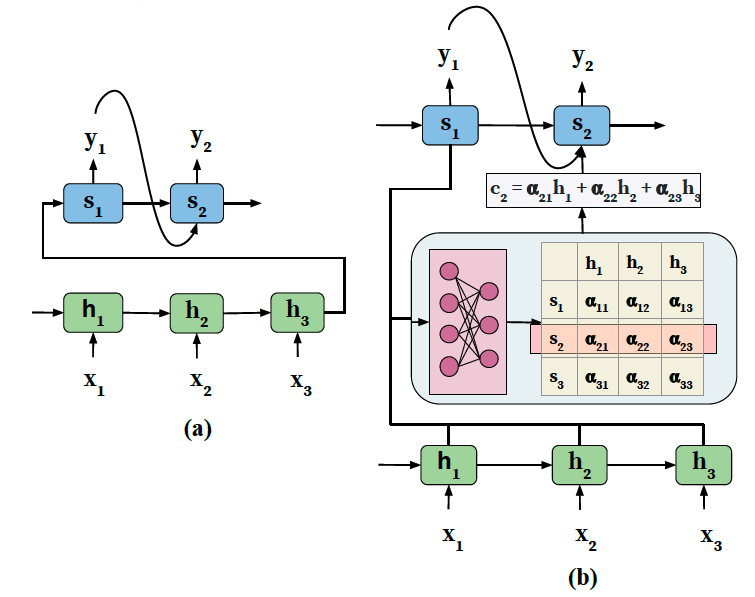
\includegraphics[width=\linewidth]{NMT.png}
  \caption{NMT architecture (a) traditional (b) with attention model.
  Figure from \cite{chaudhari1904attentive}}
  \label{NMT}
\end{figure}

In another influential paper by Xu et al \cite{xu2015show}, attention model is applied to generate caption from images. 
In this task, convolutional neural networks (CNN) is used as an encoder to extract features from raw images.
Then a long short-term memory network (LSTM) is used to generate the words, conditioned on the attention weights.
Figure \ref{attention} demonstrate how the model learn to attend to specific part of the image with the corresponding word. 
Also proposed in \cite{xu2015show}, the attention models can be classified in two types: soft and hard attention. 
In soft attention, the model is smooth and differentiable end to end, and the context vector is computed by the weighted average of the whole image. 
In contrast, in hard attention, the context vector is computed from stochastically sampled patch of image. 
The hard attention model can be faster when making inference, however, they are difficult to optimized, and require reinforcement learning to train.

\begin{figure}[htb]
  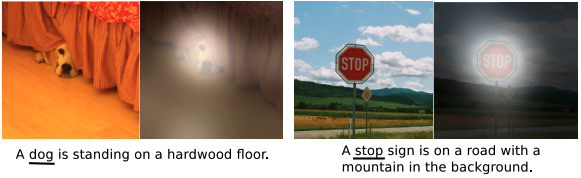
\includegraphics[width=\linewidth]{attention.png}
  \caption{Visualization of the attended region conditioned on the corresponding word.
  Figure from \cite{xu2015show}}
  \label{attention}
\end{figure}

\subsection{Memory Augmented Neural Networks}
Similar to human, in order to retrieve the information necessary for the desired tasks, a machine needs to maintain some memory that needs to be efficiently organized and queried. 
This is particularly essential for complex tasks, such as multi-hop reasoning. Traditional RNN and its variant LSTM can memorize information in the hidden states,
however, they are limited to only short term dependencies. Recent approaches to alleviate this issues involves explicit memory representation and the use of external memory, 
as proposed in Neural Turing Machine \cite{graves2014neural} and Memory Networks \cite{weston2014memory}.

A Neural Turing Machine (NTM) contains two major components: a neural network controller and a memory bank (Figure \ref{NTM}). 
A controller can be any type of neural networks, feed forward or RNN, and is responsible for read and write operations on the memory matrix.
The read and write operations are done selectively by soft attention mechanism, making every components fully differentiable, 
and thereby the whole model can be trained using gradient descent. The experiments reported in \cite{graves2014neural} have shown that NTM significantly
outperforms traditional LSTM in tasks, such as copying and sorting. Memory networks \cite{graves2014neural} are similar to NTM in the sense that they both utilise external memory, attention mechanism to select information from memory, and
can be trained end to end with gradient based learning. However, one major difference is that the memory cells in the memory networks are more static, 
as controller in memory networks only allowed read operation.

\begin{figure}[htb]
  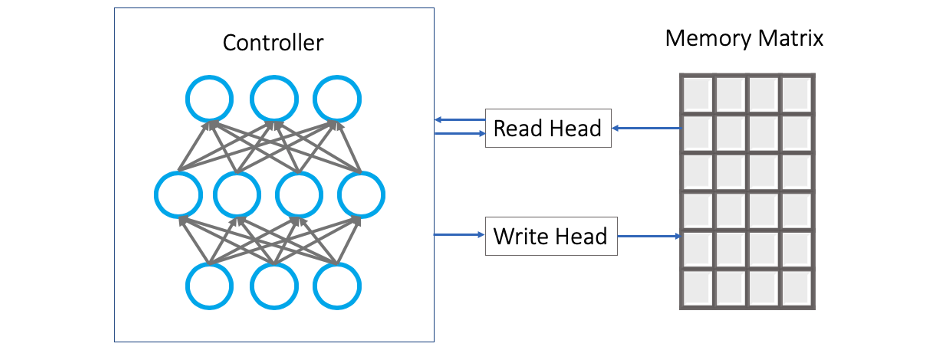
\includegraphics[width=\linewidth]{NTM.png}
  \caption{Architecture of Neural Turing Machine}
  \label{NTM}
\end{figure}

Another recent neural networks model, utilizing both attention and memory, designed to facilitate explicit reasoning is the MAC networks \cite{hudson2018compositional}.
In contrast to NTM, the MAC networks don't utilizing a global external memory. Instead, each node (MAC cell) is recurrent, and has its own memory and control state.
In contrast to traditional neural networks, the separation between control and memory encourages the networks to 
learn the computational process and reasoning operations, rather than to approximate direct transformation between the input and output.
Figure \ref{mac-clevr} shows the result of the MAC networks from a visual reasoning task using CLEVR data set \cite{johnson2017clevr}. 
The MAC networks was able to achieve 98.94\% accuracy, halving the error rate from the best prior model.
\begin{figure}[htb]
  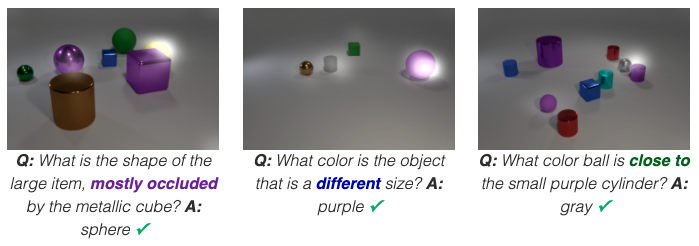
\includegraphics[width=\linewidth]{mac-clevr.png}
  \caption{Example of MAC networks performing novel visual reasoning task. Figure from \cite{hudson2018compositional}}
  \label{mac-clevr}
\end{figure}

\subsection{Graph Neural Networks}

\subsection{Neural-Symbolic}

In contrast to the purely sub-symbolic systems mention in the previous approaches, neural-symbolic is the subfield that try to integrate symbolic AI with the deep learning system. 
The idea is that the symbolic part world help the system logically reason about symbols, which is what traditional neural networks are weak at, 
while the neural network part would allow the system to learn, which the symbolic AI is not capable of.

In a visual question answering (VQA) task, recent neural-symbolic systems: NS-VQA \cite{nsvqa} and NS-CL \cite{Mao2019NeuroSymbolic} employed deep representation learning
for visual recognition and language understanding, while the reasoning part is solved by symbolic program execution.
The framework proposed in NS-CL contains three separate modules: 
a visual module where the objects are detected and vector representations are extracted, 
a semantic parser where the question text is parsed into a tree of predefined domain specific language (DSL) of executable program,
and a symbolic program executer which take in the parsed program and vector representation of objects to derive the answer. 
It has been shown that this method requires significantly less amount of training data to accurately answer questions, 
and was able to generalize to new scenes and questions better than traditional neural networks based method. 
Another added benefit of the neural-symbolic system is that the results are fully interpretable, as the execution trace is available.
Figure \ref{nscl} shows the result of this model on the VQS dataset, with the generated symbolic program.

\begin{figure}[htb]
  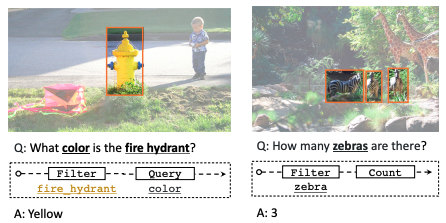
\includegraphics[width=\linewidth]{nscl.png}
  \caption{Result of NS-CL on the VQS dataset. Figure from \cite{Mao2019NeuroSymbolic}}
  \label{nscl}
\end{figure}

\section{Discussion}

\section{Conclusion}

\bibliographystyle{IEEEtran}
\bibliography{references}


\end{document}


